\chapter{La combustión: combustibles, productos y gases de efecto invernadero}\label{ch:g8:combustion-and-fuels}

Una familia duerme en un piso cuya caldera de gas tiene la salida de
humos obstruida. La llama, sin \omterm{def:g4:air-a-mixture-of-gases:air}{aire} suficiente, \omterm{def:g4:what-a-fire-needs:burning}{arde} mal, y un gas
invisible y sin olor va llenando poco a poco las habitaciones. A las dos
de la madrugada, una cajita en la pared empieza a pitar: el detector de
monóxido de carbono. Todos salen a tiempo. El mismo \omterm{def:g4:what-a-fire-needs:fuel}{combustible}, si \omterm{def:g4:what-a-fire-needs:burning}{arde}
bien, solo da dióxido de carbono y agua, y ese dióxido de carbono tiene
su propia historia, escrita en el \omterm{def:g4:air-a-mixture-of-gases:air}{aire} de todo el planeta.

\begin{recall}
Una \omterm{def:g4:what-a-fire-needs:burning}{combustión} necesita un \omterm{def:g4:what-a-fire-needs:fuel}{combustible}, oxígeno y calor, y produce
sustancias nuevas (\cref{ch:g4:what-a-fire-needs}). El \omterm{def:g4:air-a-mixture-of-gases:air}{aire} es más o
menos una quinta parte de oxígeno (\cref{ch:g4:air-a-mixture-of-gases}).
Una ecuación está ajustada cuando cada clase de \omterm{def:g7:atoms-and-molecules:atom}{átomo} aparece el mismo
número de veces en los dos miembros
(\cref{ch:g8:balanced-equations}).
\end{recall}

\section{La combustión del carbono y del metano}

\begin{example}[Dos combustiones]\label{ex:g8:combustion-and-fuels:two}
El carbono (carbón vegetal, carbón mineral) \omterm{def:g4:what-a-fire-needs:burning}{arde} y da dióxido de
carbono:
\[
  \ce{C(s) + O2(g) -> CO2(g)}.
\]
El metano, la parte principal del gas natural, \omterm{def:g4:what-a-fire-needs:burning}{arde} y da dióxido de
carbono y agua:
\[
  \ce{CH4(g) + 2O2(g) -> CO2(g) + 2H2O(l)}.
\]
En los dos casos, el gas formado enturbia el agua de cal; con el metano,
además, un vaso frío se empaña.
\end{example}

\begin{method}[Escribir la combustión de un combustible formado por carbono e hidrógeno]\label{met:g8:combustion-and-fuels:write}
Para un \omterm{def:g4:what-a-fire-needs:fuel}{combustible} cuyas \omterm{def:g7:atoms-and-molecules:molecule}{moléculas} solo contienen carbono e hidrógeno:
\begin{enumerate}
  \item los productos son el dióxido de carbono y el agua;
  \item se ajusta el carbono con \ce{CO2} y después el hidrógeno con
        \ce{H2O};
  \item se cuentan los \omterm{def:g7:atoms-and-molecules:atom}{átomos} de oxígeno de la derecha y se ajustan con
        \ce{O2}; si aparece una mitad, se duplica todo.
\end{enumerate}
Para el butano: \ce{2C4H10 + 13O2 -> 8CO2 + 10H2O}.
\end{method}

\section{Combustión completa e incompleta}

\begin{definition}[Combustión completa e incompleta]\label{def:g8:combustion-and-fuels:complete}
Una \emph{combustión completa}\index{combustion completa@combustión completa} se produce
con oxígeno suficiente: todo el carbono del \omterm{def:g4:what-a-fire-needs:fuel}{combustible} se convierte en
dióxido de carbono. Una
\emph{combustión incompleta}\index{combustion incompleta@combustión incompleta} se produce
con demasiado poco oxígeno: parte del carbono se convierte en monóxido
de carbono, \ce{CO}, o en hollín, que es carbono, \ce{C}.
\end{definition}

\begin{example}[Metano con poco oxígeno]\label{ex:g8:combustion-and-fuels:incomplete}
Con demasiado poco \omterm{def:g4:air-a-mixture-of-gases:air}{aire}, el metano puede \omterm{def:g4:what-a-fire-needs:burning}{arder} dando monóxido de carbono
o hollín:
\[
  \ce{2CH4 + 3O2 -> 2CO + 4H2O}, \qquad \ce{CH4 + O2 -> C + 2H2O}.
\]
\end{example}

\begin{proposition}[Leer una llama]\label{prop:g8:combustion-and-fuels:flame}
Un mechero Bunsen con la entrada de \omterm{def:g4:air-a-mixture-of-gases:air}{aire} abierta \omterm{def:g6:pure-substances-and-mixtures:mixture}{mezcla} \omterm{def:g4:air-a-mixture-of-gases:air}{aire} con el gas
antes de que arda: la llama es azul y apenas visible, y la \omterm{def:g4:what-a-fire-needs:burning}{combustión} es
completa. Con la entrada de \omterm{def:g4:air-a-mixture-of-gases:air}{aire} cerrada, el gas encuentra demasiado
poco oxígeno: la llama es amarilla, humea y ennegrece de hollín un
objeto frío que se acerque a ella; la \omterm{def:g4:what-a-fire-needs:burning}{combustión} es incompleta.
\end{proposition}

\begin{omfigure}
\begin{tikzpicture}[font=\small, scale=1.3]
  \pic[transform shape] at (0,0) {bunsen=open};
  \node[anchor=north, align=center] at (0,-0.1) {entrada de aire abierta:\\ llama azul, completa};
  \pic[transform shape] at (4,0) {bunsen=closed};
  \node[anchor=north, align=center] at (4,-0.1) {entrada de aire cerrada:\\ llama amarilla, incompleta};
  \draw[<-, omProp, thick] (0.08,0.6) -- (1.4,0.9) node[right, text=black] {entrada de aire};
  \draw[<-, omProp, thick] (-0.4,0.3) -- (-1.3,0.6) node[left, text=black] {gas};
  \draw[<-, omProp, thick] (4.15,3.3) -- (5.0,3.5) node[right, text=black, align=left]
    {hollín, monóxido\\ de carbono};
\end{tikzpicture}

{\small Un mechero Bunsen. El \omterm{def:g4:air-a-mixture-of-gases:air}{aire} que entra por abajo da una llama azul
y una \omterm{def:g8:combustion-and-fuels:complete}{combustión completa}; sin él, la llama es amarilla y humea.}
\end{omfigure}

\begin{omfigure}
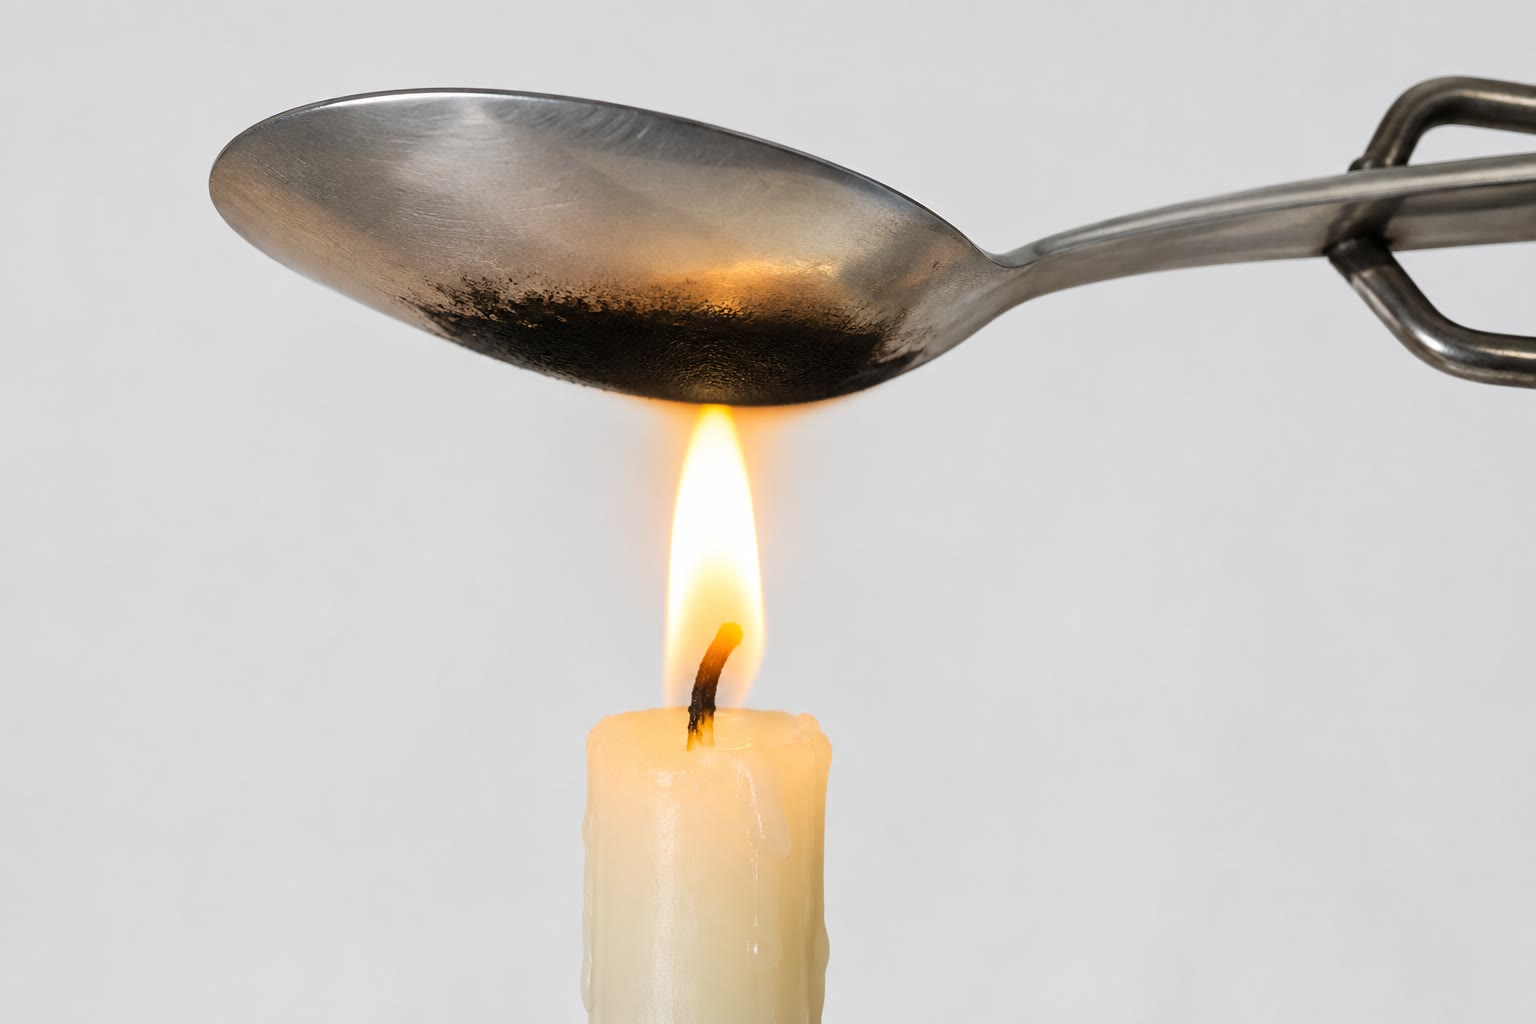
\includegraphics[width=0.45\linewidth]{images/book1/ai/g8-soot-spoon.jpg}

{\small Una cuchara fría sostenida en la llama amarilla de una vela se
ennegrece de hollín: la \omterm{def:g4:what-a-fire-needs:burning}{combustión} es incompleta.}
\end{omfigure}

\section{El monóxido de carbono, un peligro silencioso}

\begin{proposition}[Por qué mata el monóxido de carbono]\label{prop:g8:combustion-and-fuels:co}
El monóxido de carbono no tiene color, ni olor, ni sabor. Al
respirarlo, ocupa el lugar del oxígeno en la sangre (el libro de
biología explica cómo) y provoca dolor de cabeza, somnolencia y, en una
habitación cerrada, pérdida del conocimiento y la muerte. Lo produce
cualquier \omterm{def:g4:what-a-fire-needs:fuel}{combustible} que \omterm{def:g4:what-a-fire-needs:burning}{arde} con poco \omterm{def:g4:air-a-mixture-of-gases:air}{aire}: una caldera o un
calentador de gas mal revisados o con la salida de humos obstruida, un
hornillo en una tienda de campaña cerrada, una barbacoa o un generador
usados en un interior.
\end{proposition}

\begin{safety}{\ghs[0.8cm]{GHS02}\ghs[0.8cm]{GHS04}\ghs[0.8cm]{GHS06}\ghs[0.8cm]{GHS08}}
% ledger: ghs:CO
Monóxido de carbono: gas extremadamente inflamable (GHS02), suministrado
a presión (GHS04); tóxico en caso de inhalación (GHS06); perjudica a
determinados órganos por exposiciones repetidas y puede dañar al feto
(GHS08).
\end{safety}

\begin{remark}[Prevenir las intoxicaciones]\label{rem:g8:combustion-and-fuels:prevent}
Los aparatos de gas los revisa con regularidad un profesional, las
salidas de humos y las rejillas de ventilación no se tapan nunca, las
barbacoas y los generadores solo se usan al \omterm{def:g4:air-a-mixture-of-gases:air}{aire} libre, y se instala un
detector de monóxido de carbono cerca de cualquier quemador.
\end{remark}

\begin{omfigure}
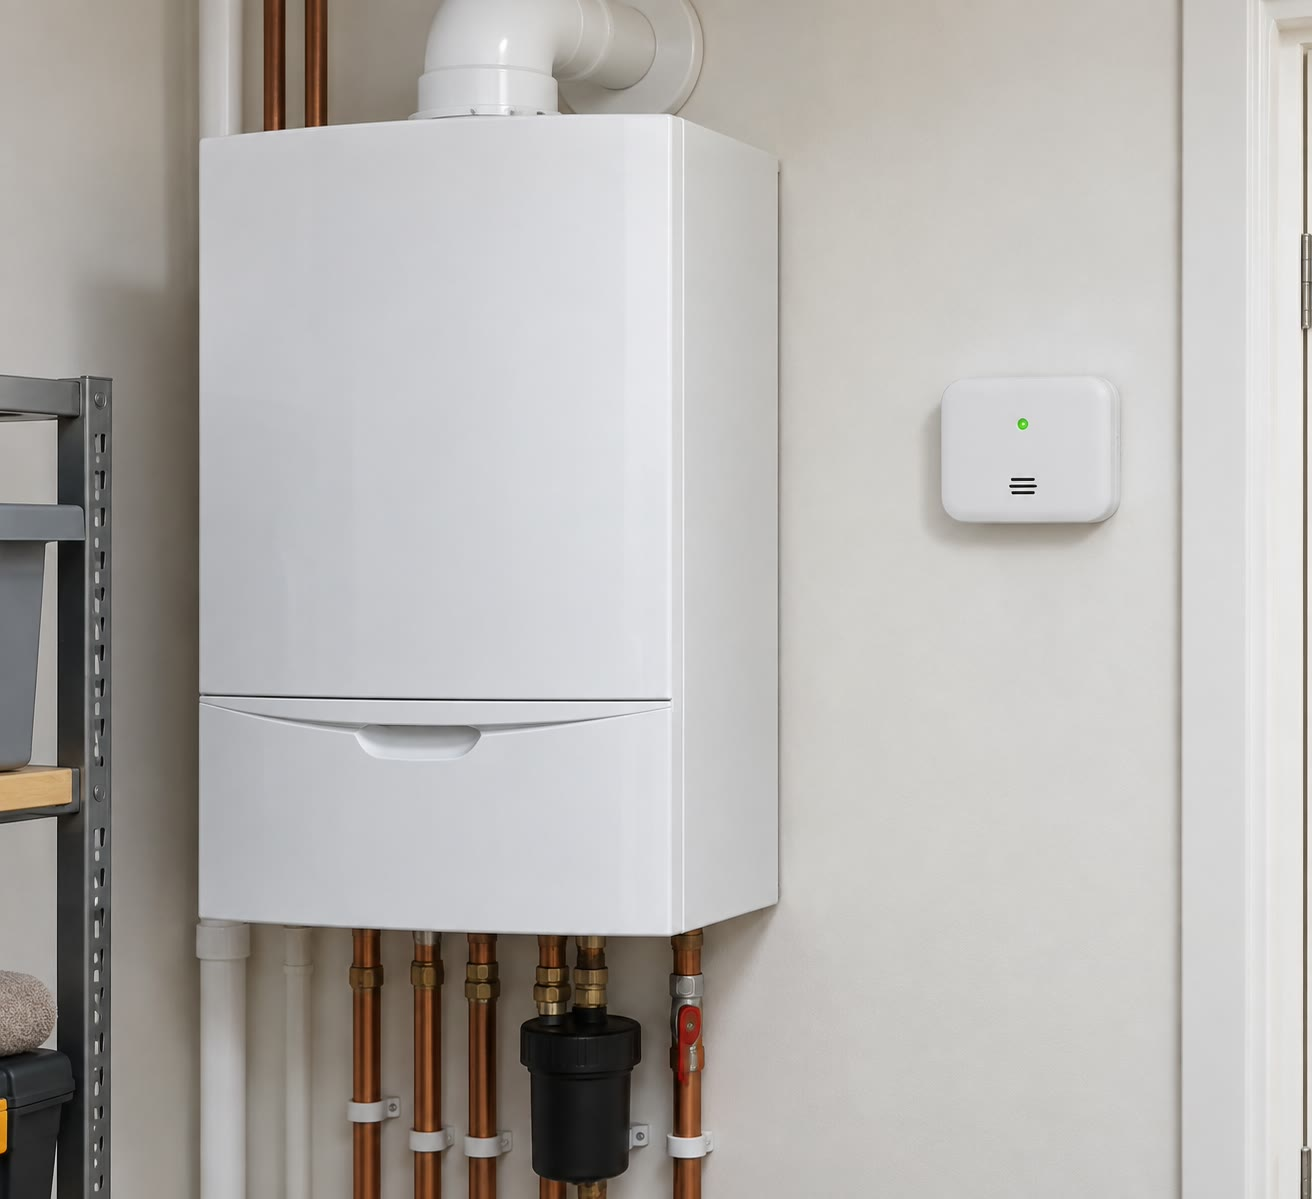
\includegraphics[width=0.45\linewidth]{images/book1/ai/g8-boiler-alarm.jpg}

{\small Una caldera de gas y, a su lado, un detector de monóxido de
carbono.}
\end{omfigure}

\section{El dióxido de carbono y el efecto invernadero}

\begin{definition}[Gas de efecto invernadero]\label{def:g8:combustion-and-fuels:greenhouse}
Un \emph{gas de efecto invernadero}\index{gas de efecto invernadero} es
un gas del \omterm{def:g4:air-a-mixture-of-gases:air}{aire} que deja pasar la luz del Sol pero retiene parte del
calor que la superficie de la Tierra devuelve hacia el espacio, y así
calienta la atmósfera baja. El vapor de agua, el dióxido de carbono y el
metano son gases de efecto invernadero; el nitrógeno y el oxígeno, no.
(Cómo ocurre esto lo explica el libro de física.)
\end{definition}

\begin{proposition}[El dióxido de carbono del aire aumenta]\label{prop:g8:combustion-and-fuels:rising}
% ledger: co2:mlo-1959, co2:mlo-2025 (rise 111.4 ppm, +35 %)
La cantidad de dióxido de carbono del \omterm{def:g4:air-a-mixture-of-gases:air}{aire} se mide sin interrupción
desde 1959 en un observatorio situado en una montaña en mitad del océano
Pacífico. Era de 316 partes por millón (ppm) de \omterm{def:g4:air-a-mixture-of-gases:air}{aire} en 1959 y de 427
ppm en 2025: un aumento de alrededor del \qty{35}{\percent} en una vida
humana, debido sobre todo a la quema de carbón, petróleo y gas natural.
El dióxido de carbono adicional refuerza el efecto invernadero y
calienta el clima.
\end{proposition}

\begin{omfigure}
\begin{tikzpicture}
\begin{axis}[width=0.85\linewidth, height=6cm, xmin=1955, xmax=2030,
    ymin=300, ymax=440, xlabel={año}, ylabel={dióxido de carbono (ppm)},
    axis lines*=left, ymajorgrids, grid style={gray!20},
    tick label style={font=\small, /pgf/number format/1000 sep={}},
    label style={font=\small}]
\addplot[omDef, thick, mark=*, mark size=0.8pt]
  table[x=year, y=ppm] {figdata/out/grade-8-co2-record.dat};
\node[anchor=west, font=\small] at (axis cs:1962,306) {316 ppm en 1959};
\node[anchor=east, font=\small] at (axis cs:2023,428) {427 ppm en 2025};
\end{axis}
\end{tikzpicture}

{\small Media anual del dióxido de carbono del \omterm{def:g4:air-a-mixture-of-gases:air}{aire}, medida desde 1959
(datos del NOAA Global Monitoring Laboratory; antes de 1974, de la
Scripps Institution of Oceanography).}
\end{omfigure}

\section{Combustibles fósiles y renovables}

\begin{definition}[Combustibles fósiles y renovables]\label{def:g8:combustion-and-fuels:fossil}
Un \emph{combustible fósil}\index{combustible fosil@combustible fósil} (el carbón, el
petróleo, el gas natural) se formó bajo tierra a lo largo de millones de
años a partir de los restos de plantas y animales marinos antiguos. Un
\emph{combustible renovable}\index{combustible renovable} se obtiene de
plantas cultivadas hoy, o de residuos: la madera, el biogás del
estiércol y de los restos de comida, el etanol fabricado con remolacha
o caña de azúcar.
\end{definition}

\begin{proposition}[De dónde viene el carbono]\label{prop:g8:combustion-and-fuels:cycle}
Las plantas toman dióxido de carbono del \omterm{def:g4:air-a-mixture-of-gases:air}{aire} para crecer. Quemar un
\omterm{def:g8:combustion-and-fuels:fossil}{combustible renovable} devuelve el dióxido de carbono que sus plantas
tomaron del \omterm{def:g4:air-a-mixture-of-gases:air}{aire} hace pocos años. Quemar un \omterm{def:g8:combustion-and-fuels:fossil}{combustible fósil} libera
carbono que estuvo encerrado bajo tierra durante millones de años: añade
dióxido de carbono al \omterm{def:g4:air-a-mixture-of-gases:air}{aire}.
\end{proposition}

\begin{omfigure}
\begin{tikzpicture}[font=\small,
    box/.style={draw=omDef, fill=omDef!6, rounded corners=2pt, align=center,
      minimum height=0.9cm, text width=2.6cm}]
  \node[box] (air) at (0,3) {dióxido de carbono\\ en el aire};
  \node[box] (plants) at (5.6,3) {las plantas crecen\\ (toman \ce{CO2})};
  \node[box] (fuel) at (5.6,0.4) {madera, biogás,\\ bioetanol};
  \node[box, draw=black!50, fill=black!8] (fossil) at (0,0.4) {carbón, petróleo, gas:\\ bajo tierra};
  \draw[->, thick, omProp] (air) -- (plants);
  \draw[->, thick, omProp] (plants) -- (fuel);
  \draw[->, thick, omProp] (fuel) -- (air);
  \node[text=black, font=\footnotesize, align=left, anchor=north west] at (1.5,1.45)
    {combustión,\\ pocos años después};
  \draw[->, thick, black!60] (fossil) -- node[midway, left, text=black, font=\footnotesize,
    align=right] {combustión:\\ carbono almacenado\\ durante millones\\ de años} (air);
\end{tikzpicture}

{\small Los \omterm{def:g8:combustion-and-fuels:fossil}{combustibles renovables} devuelven al \omterm{def:g4:air-a-mixture-of-gases:air}{aire} el carbono que sus
plantas le tomaron; los \omterm{def:g8:combustion-and-fuels:fossil}{combustibles fósiles} añaden carbono que estaba
almacenado bajo tierra.}
\end{omfigure}

\begin{omfigure}
\begin{minipage}[t]{0.48\linewidth}\centering
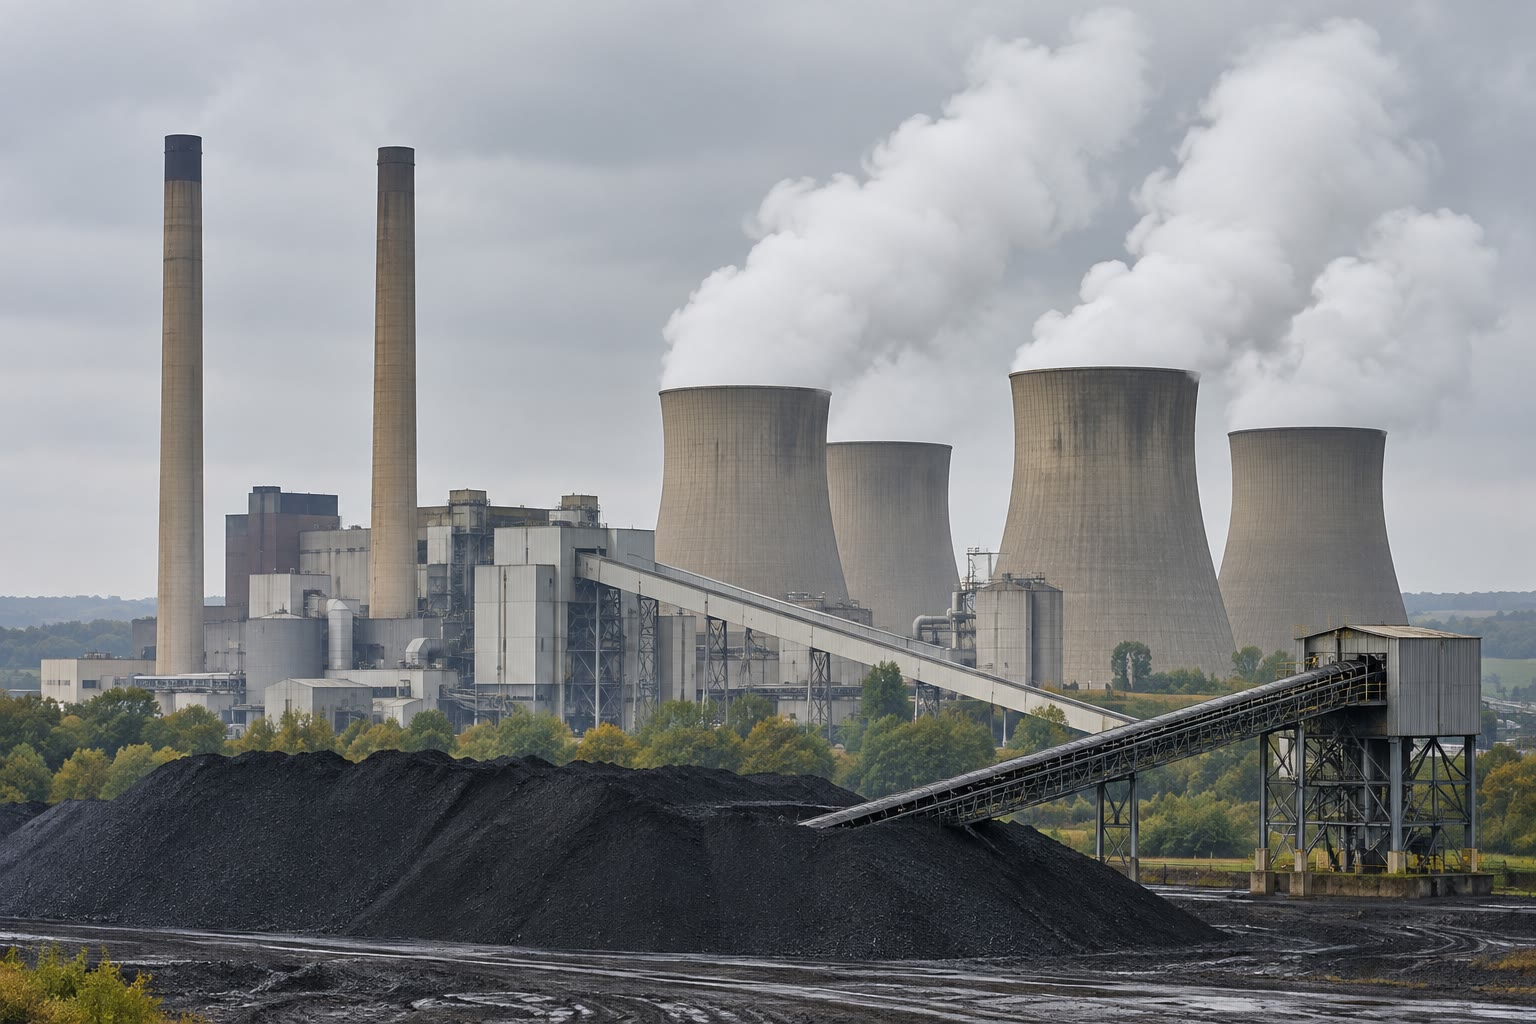
\includegraphics[width=\linewidth,height=4.6cm,keepaspectratio]{images/book1/ai/g8-coal-plant.jpg}

{\small Una central térmica de carbón.}
\end{minipage}\hfill
\begin{minipage}[t]{0.48\linewidth}\centering
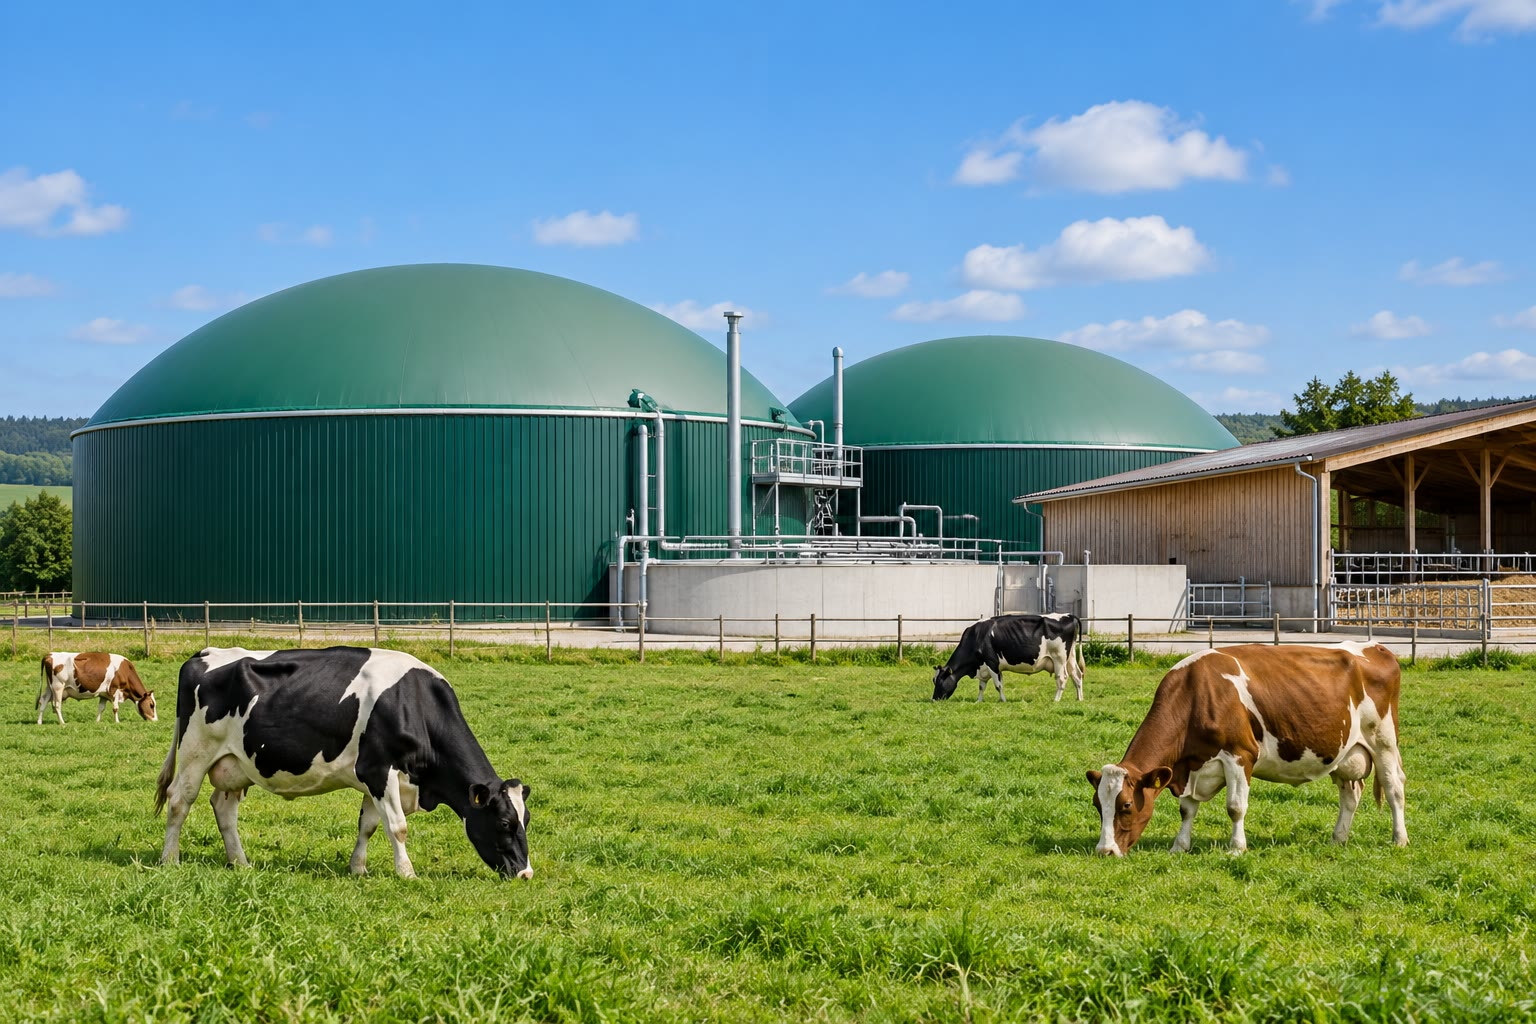
\includegraphics[width=\linewidth,height=4.6cm,keepaspectratio]{images/book1/ai/g8-biogas-farm.jpg}

{\small Una planta de biogás en una granja: el estiércol se convierte en
un \omterm{def:g8:combustion-and-fuels:fossil}{combustible renovable}.}
\end{minipage}
\end{omfigure}

\section{Ejercicios}

\begin{exercise}[$\star$]\label{exo:g8:combustion-and-fuels:1}
Escribe la \omterm{def:g8:balanced-equations:equation}{ecuación ajustada} de la \omterm{def:g8:combustion-and-fuels:complete}{combustión completa} del carbono.
\end{exercise}

\begin{exercise}[$\star$]\label{exo:g8:combustion-and-fuels:2}
¿Qué diferencia hay entre una \omterm{def:g8:combustion-and-fuels:complete}{combustión completa} y una incompleta?
\end{exercise}

\begin{exercise}[$\star$]\label{exo:g8:combustion-and-fuels:3}
¿Por qué se dice que el monóxido de carbono es un peligro silencioso?
\end{exercise}

\begin{exercise}[$\star$]\label{exo:g8:combustion-and-fuels:4}
¿Fósil o renovable: el carbón, la madera, el gas natural, el biogás, la
gasolina, el etanol de remolacha?
\end{exercise}

\begin{exercise}[$\star\star$]\label{exo:g8:combustion-and-fuels:5}
Escribe la \omterm{def:g8:balanced-equations:equation}{ecuación ajustada} de la \omterm{def:g8:combustion-and-fuels:complete}{combustión completa} del propano,
\ce{C3H8}.
\end{exercise}

\begin{exercise}[$\star\star$]\label{exo:g8:combustion-and-fuels:6}
El etanol, \ce{C2H6O}, \omterm{def:g4:what-a-fire-needs:burning}{arde} por completo en oxígeno. Ajusta
\ce{C2H6O + O2 -> CO2 + H2O}. % ce-unbalanced-ok (to balance)
\end{exercise}

\begin{exercise}[$\star\star$]\label{exo:g8:combustion-and-fuels:7}
Una cazuela sostenida sobre una llama amarilla se ennegrece por debajo.
¿Qué es la sustancia negra? ¿Qué nos dice sobre la \omterm{def:g4:what-a-fire-needs:burning}{combustión}?
\end{exercise}

\begin{exercise}[$\star\star$]\label{exo:g8:combustion-and-fuels:8}
Lee la curva del dióxido de carbono: ¿cuánto dióxido de carbono, más o
menos, contenía el \omterm{def:g4:air-a-mixture-of-gases:air}{aire} en 1980 y en 2000? ¿Cuántas ppm aumentó en esos
veinte años?
\end{exercise}

\begin{exercise}[$\star\star$]\label{exo:g8:combustion-and-fuels:9}
¿Por qué quemar madera añade, con los años, menos dióxido de carbono al
\omterm{def:g4:air-a-mixture-of-gases:air}{aire} que quemar carbón, aunque los dos den dióxido de carbono?
\end{exercise}

\begin{exercise}[$\star\star$]\label{exo:g8:combustion-and-fuels:10}
Ajusta la \omterm{def:g8:combustion-and-fuels:complete}{combustión incompleta} del carbono que da monóxido de carbono,
\ce{C + O2 -> CO}. % ce-unbalanced-ok (to balance)
\end{exercise}

\begin{exercise}[$\star\star\star$]\label{exo:g8:combustion-and-fuels:11}
De 1959 (316 ppm) a 2025 (427 ppm), ¿en qué porcentaje aumentó el
dióxido de carbono del \omterm{def:g4:air-a-mixture-of-gases:air}{aire}? Redondea al número entero más próximo.
\end{exercise}

\begin{exercise}[$\star\star\star$]\label{exo:g8:combustion-and-fuels:12}
Se usa una estufa de gas en una habitación pequeña con la ventana
cerrada. Explica, con dos ecuaciones de este capítulo, cómo la
\omterm{def:g4:what-a-fire-needs:burning}{combustión} puede pasar de completa a incompleta a medida que pasa el
tiempo, y por qué esto es peligroso.
\end{exercise}

\section{Problema: El hornillo en la tienda de campaña}

\begin{problem}[{Problema de fin de semana --- un hornillo de camping,
el gas que quema, lo que produce y por qué nunca se mete en una tienda
de campaña}]
\label{pb:g8:combustion-and-fuels:1}
% ledger: ghs:propane
Un hornillo de camping quema propano, \ce{C3H8}, de un cartucho que
contiene \qty{450}{g}. Al \omterm{def:g4:air-a-mixture-of-gases:air}{aire} libre, la llama es azul. Toma estas
proporciones en masa, calculadas a partir de la \omterm{def:g8:balanced-equations:equation}{ecuación ajustada}:
\qty{44}{g} de propano que \omterm{def:g4:what-a-fire-needs:burning}{arden} por completo dan \qty{132}{g} de
dióxido de carbono.

\medskip
\noindent\textbf{Parte I --- Las ecuaciones.}
\begin{enumerate}
  \item Escribe la \omterm{def:g8:balanced-equations:equation}{ecuación ajustada} de la \omterm{def:g8:combustion-and-fuels:complete}{combustión completa} del
        propano.
  \item Compruébala contando los \omterm{def:g7:atoms-and-molecules:atom}{átomos} de cada clase en cada miembro.
  \item Ajusta la \omterm{def:g8:combustion-and-fuels:complete}{combustión incompleta}
        \ce{C3H8 + O2 -> CO + H2O}. % ce-unbalanced-ok (to balance)
  \item ¿Cuál de las dos necesita más oxígeno por \omterm{def:g7:atoms-and-molecules:molecule}{molécula} de propano?
\end{enumerate}

\medskip
\noindent\textbf{Parte II --- Dentro de una tienda de campaña.}
\begin{enumerate}[resume]
  \item Un hornillo encendido dentro de una tienda cerrada pronto \omterm{def:g4:what-a-fire-needs:burning}{arde}
        con una llama amarilla. Explica por qué.
  \item ¿Qué gas peligroso se forma entonces? Da dos de sus propiedades
        que hacen difícil notarlo.
  \item El cartucho de propano lleva dos pictogramas. Nómbralos y di qué
        significa cada uno.
  \item Da dos normas para usar un hornillo de camping con seguridad.
\end{enumerate}

\medskip
\noindent\textbf{Parte III --- El dióxido de carbono de un cartucho.}
\begin{enumerate}[resume]
  \item ¿Cuántas veces más pesa el dióxido de carbono formado que el
        propano quemado?
  \item ¿De dónde salen los gramos adicionales?
  \item ¿El propano es un \omterm{def:g8:combustion-and-fuels:fossil}{combustible fósil} o renovable? ¿Al quemarlo se
        añade dióxido de carbono al \omterm{def:g4:air-a-mixture-of-gases:air}{aire}?
  \item Calcula la masa de dióxido de carbono liberada cuando \omterm{def:g4:what-a-fire-needs:burning}{arde} por
        completo un cartucho entero de \qty{450}{g}.
\end{enumerate}
\end{problem}
